\subsubsection{Attività}
\label{sec:4.1.1}
	\paragraph{Comunicazioni}
	\label{sec:4.1.1.1}
		\subparagraph{Comunicazioni interne}
		\label{sec:4.1.1.1.1}
			Per le comunicazioni interne si è deciso di utilizzare \gl{Slack}. Sono stati creati diversi canali per suddividere il lavoro. I canali sono:
			\begin{itemize}
				\item \textit{\#general}: in questo canale va utilizzato per le comunicazioni di carattere generale e per le convocazioni delle riunioni; 
				\item \textit{\#random}: in caso di piccoli dubbi o questioni di scarsa rilevanza, si consiglia l'utilizzo di questo canale; 
				\item \textit{\#tools}: questo canale è stato creato per domande relative a dubbi e/o problemi sugli strumenti utilizzati per lo sviluppo;
				\item \textit{\#\gl{git}}: su questo canale è stato collegato un \gl{bot} che si occupa di notificare tutti i \gl{commit} effettuati da ogni singolo componente del gruppo;
				\item \textit{\#nome\_del\_documento}: per ogni documento è stato creato un canale dove è possibile discutere di tutte le scelte da prendere per quel singolo documento.
			\end{itemize}
			In caso di necessità, sarà possibile aggiungere nuovi canali nelle fasi successive dello sviluppo. \\
			Inoltre è possibile utilizzare il gruppo creato su \gl{Telegram} per comunicazioni interne non inerenti al \gl{progetto}. Per le videoconferenze invece verrà utilizzato \gl{Google Hangouts}.
		\subparagraph{Comunicazioni esterne}
		\label{sec:4.1.1.1.2}
			Per le comunicazioni esterne è stata creata la casella di posta elettronica: \\
			\highlight{\EMAIL}\\
			Questo indirizzo deve essere l'unico usato per comunicare con le componenti esterne al team ed è controllato unicamente dal \RES. Il \RES  \ è tenuto poi ad informare i membri del team riguardo le comunicazioni avvenute con l'esterno.
	\paragraph{Riunioni}
	\label{sec:4.1.1.2}
		\subparagraph{Riunioni interne}
		\label{sec:4.1.1.2.1}
			Il gruppo si ritroverà ad organizzare una riunione almeno ogni dieci giorni. \\
			Il \RES \ si occuperà di convocare su \gl{Slack} le riunioni generali cui tutti i membri del team sono convocati, avvisando i componenti con almeno due giorni di preavviso. \\
			In caso di necessità un componente del team può richiedere la convocazione di una riunione: tale richiesta deve essere inoltrata al \RES, che deciderà se accettarla o respingerla. \\
			Inoltre sono possibili riunioni tra specifici membri: in questo caso sono tenuti ad informare il resto del team tramite un verbale, nel caso siano state prese decisioni rilevanti. \\
		\subparagraph{Riunioni esterne}
		\label{sec:4.1.1.2.2}
			Il \RES  \ si occuperà di concordare con il \gl{proponente} o con i committenti le riunioni esterne al gruppo. È gradita la presenza di tutti i componenti del gruppo ad ogni incontro. \\
			Prima dell'inizio di ogni riunione verrà scelto un componente del gruppo che svolgerà la funzione di segretario, il quale annoterà ogni argomento trattato e si occuperà di redigere un verbale che andrà poi inviato agli altri componenti del team.
	\paragraph{Ticket}
	\label{sec:4.1.1.3}
		I \gl{ticket} avranno la seguente struttura:
		\begin{itemize}
		 	\item \textbf{Titolo}: deve rappresentare in modo chiaro e conciso il \gl{task};
		 	\item \textbf{Scadenza}: data entro cui l'assegnatario deve concludere il \gl{task};
		 	\item \textbf{Descrizione}: se necessario,deve chiarire con una breve descrizione il \gl{task};
		 	\item \textbf{Assegnatario}: colui che dovrà completare il \gl{task};
		 	\item \textbf{Tag di stato}: deve contenere il giusto tag che rappresenta lo stato attuale del \gl{task}; 
		 	\item \textbf{Subtasks}: il \gl{task} può essere suddiviso in \gl{task} piu piccoli.
		 	\end{itemize}
	 	\subparagraph{Lista dei tag}
	 	\label{sec:4.1.1.3.1}
		 	Ogni \gl{ticket} dovrà sempre contenere un tag che rappresenti lo stato attuale di avanzamento:
		 	\begin{itemize}
		 		\item \textbf{Assegnato}: il \gl{ticket} è stato assegnato ad un membro del team;
		 		\item \textbf{Accettato}: l'assegnatario ha preso in carico il \gl{ticket};
		 		\item \textbf{Rifiutato}: l'assegnatario ha rifiutato il \gl{ticket} ed ha inserito la motivazione in un commento;
		 		\item \textbf{InCorso}: l'assegnatario sta svolgendo il \gl{task};
		 		\item \textbf{InSospeso}: l'assegnatario specifica della motivazione per cui ha messo in attesa il \gl{ticket};
		 		\item \textbf{Completato}: l'assegnatario ha concluso il \gl{task};
		 		\item \textbf{Verificato}: il \gl{ticket} è stato verificato.
		 		\end{itemize}
\subsubsection{Procedure}
\label{sec:4.1.2}
	\paragraph{Creazione di un \gl{ticket}}
	\label{sec:4.1.2.1}
		La creazione e l'assegnazione dei \gl{ticket} sarà delegata al Responsabile che seguirà la seguente procedura:
		\begin{itemize}
			\item assegna il \textbf{titolo} del \gl{ticket};
			\item assegna la data di \textbf{scadenza} del \gl{ticket};
			\item se necessario descrive il \gl{task} più approfonditamente tramite la \textbf{descrizione};
			\item assegna il \gl{ticket} ad un \textbf{assegnatario};
			\item imposta il \textbf{tag di stato} ad \textbf{Assegnato}.
		\end{itemize}
		\begin{figure}
			\centering
			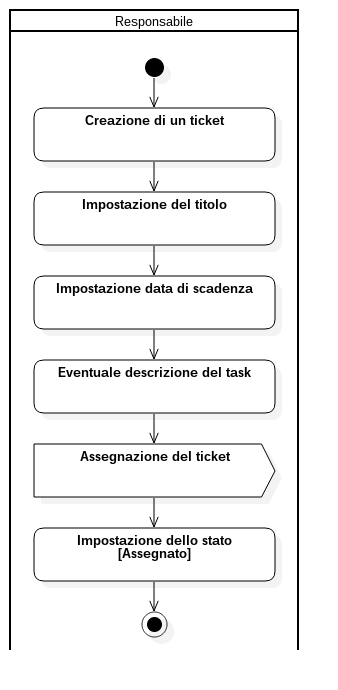
\includegraphics[scale=0.80]{img/creazioneTicket.png}
			\caption{Creazione di un \gl{ticket}}
		\end{figure}
	\paragraph{Aggiornamento di un \gl{ticket}}
	\label{sec:4.1.2.2}
		Ogni membro del gruppo avrà una lista di \gl{ticket} a lui assegnati, su di essi dovrà modificare il tag di stato ogni qual volta uno di questi cambi di stato come descritto dalla sezione 4.1.1.3.1. Nel caso in cui il \gl{ticket} venga \textbf{rifiutato} o venga messo \textbf{in sospeso} è necessario scrivere una motivazione attraverso un commento.
		\begin{figure}
			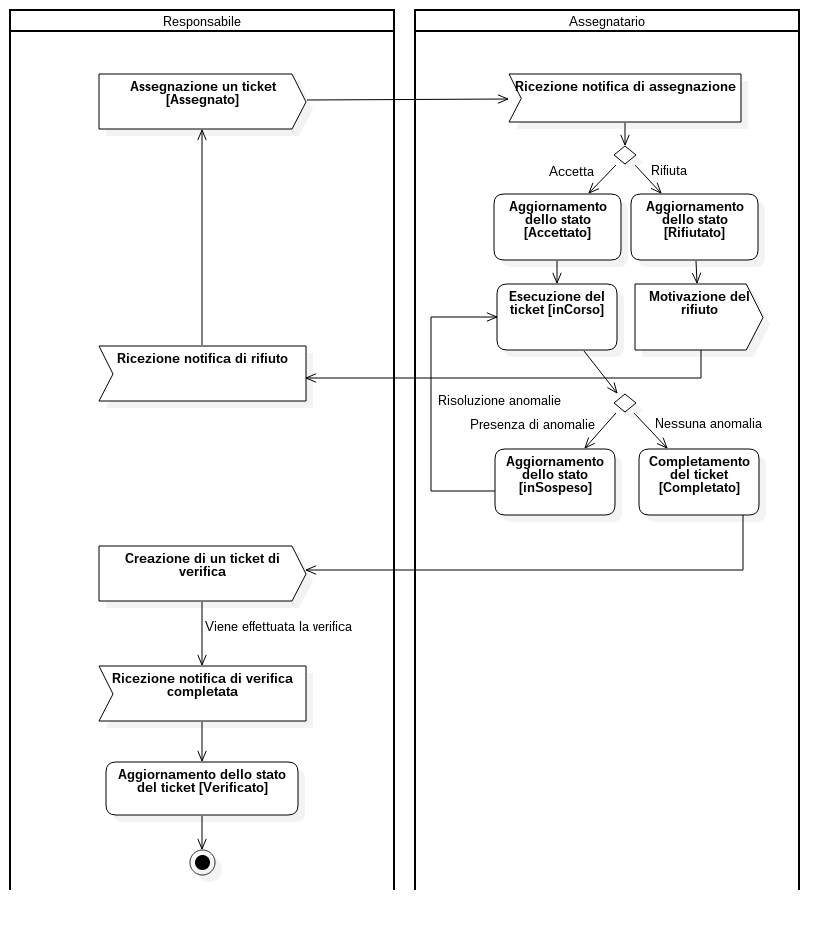
\includegraphics[scale=.53]{img/vitaTicket.png}
			\centering
			\caption{Ciclo di vita di un \gl{ticket}}
		\end{figure}
\subsubsection{Norme}
\label{sec:4.1.3}
	\paragraph{\gl{Repository}}
	\label{sec:4.1.3.1}
		Per la gestione condivisa e per il controllo delle versioni dei file il \gl{team} ha deciso di utilizzare una \gl{repository} fornita dal servizio web \gl{GitHub}.
		\subparagraph{Struttura del \gl{repository}}
		\label{sec:4.1.3.1.1}
			La respository si divide in due cartelle principali:
			\begin{itemize}
				\item \textbf{Codice}: contenente il codice del \gl{progetto}, con struttura ancora da definire;
				\item \textbf{Documenti}: contenente:
				\begin{enumerate}
					\item \textbf{\gl{template}}: con al suo interno i file \file{.sty} e una cartella \textbf{img} contenente le immagini (vedi sezione 3.1.2.1);
					\item \textbf{\gl{script}}: con al suo interno gli \gl{script};
					\item una cartella per ogni \textbf{revisione di avanzamento}, il cui nome è definito dal numero e dalla sigla della revisione, separata da un trattino. Ciascuna di esse è suddivisa in:
					\begin{enumerate}
						\item \textbf{interni}: contenente una cartella per ogni documento interno, con nome, in notazione \gl{CamelCase}, uguale a quello del documento(senza numero di versione);
						\item \textbf{esterni}: contenente una cartella per ogni documento esterno, con nome, in notazione \gl{CamelCase}, uguale a quello del documento(senza numero di versione);
					\end{enumerate}
					Ogni cartella dei documenti ha al suo interno, se necessario, una cartella \textbf{img} contenente le immagini e i diagrammi presenti in quel documento.
				\end{enumerate}
			\end{itemize}
		\subparagraph{Tipi di file e .gitignore}
		\label{sec:4.1.3.1.2}
			All'interno delle cartelle dei documenti saranno presenti solamente i file \file{.tex}, i restanti file ausiliari prodotti da \gl{\LaTeX} sono stati aggiunti a .gitignore e quindi vengono ignorati e resi invisibili da \gl{Git}.
		\subparagraph{Norme sulla \gl{commit}}
		\label{sec:4.1.3.1.3}
			Per rendere effettive le modifiche applicate ai file della \gl{repository} locale è necessario eseguire una \textbf{\gl{commit}}.
			I membri del team sono tenuti ad effettuare una \gl{commit} ogni qual volta venga aggiunta, rimossa o aggiornata una funzionalità oppure una sezione, aggiungendo i file interessati tramite il commando:
			\begin{center}
				\file{\gl{git} add nome\_del\_file.est}
			\end{center}
			ed eseguendo la \gl{commit} tramite il commando:
			\begin{center}
				\file{\gl{git} \gl{commit} -m ``messaggio''}
			\end{center}
			con \file{messaggio} che segua le regole della sezione 3.2.1.
			Infine per rendere effettive le modifiche nel \gl{repository} in remoto eseguire:
			\begin{center}
				\file{\gl{git} \gl{push}}
			\end{center}
		\subparagraph{Messaggi delle \gl{commit}}
		\label{sec:4.1.3.1.4}
			Ogni qual volta venga eseguita una \file{\gl{commit}} è obbligatorio inserire un breve messaggio con la spiegazione
			delle modifiche apportate; il messaggio deve iniziare con:
			\begin{itemize}
				\item \textbf{Add:} se vengono aggiunte funzionalità o sezioni;
				\item \textbf{Remove:} se vengono tolte funzionalità o sezioni;
				\item \textbf{Update:} se vendono aggiornate funzionalità o sezioni;
				\item \textbf{Fix:} se viene sistemato un bug noto;
			\end{itemize}
			deve seguire una descrizione sintetica in lingua italiana delle modifiche apportate.
\subsubsection{Strumenti}
\label{sec:4.1.4}
	\paragraph{Sistema operativo}
	\label{sec:4.1.4.1}
		Non ci sono restrizioni riguardo l'utilizzo di un sistema operativo: ogni membro del team può utilizzare quindi il sistema operativo che preferisce; in ogni caso, è tenuto a rendere il materiale \gl{prodotto} \textbf{completamente} compatibile su tutte le piattaforme.
	\paragraph{Condivisione}
	\label{sec:4.1.4.2}
		Il servizio da utilizzare per i documenti informali è \gl{Google Drive}.
		All'interno di questo \gl{repository} vanno caricati documenti che:
		\begin{itemize}
			\item non necessitano di controllo di versione;
			\item necessitano di essere modificati contemporaneamente da più persone; infatti \gl{Google Drive} permette la modifica di un documento in contemporanea: in questo modo non ci saranno conflitti.
		\end{itemize}
		È possibile anche condividere link o manuali utili per la formazione del team. Si può installare \gl{Google Drive} sul proprio PC: i file così potranno essere disponibili anche offline e sincronizzare il contenuto della cartella ad ogni aggiornamento.
	\paragraph{Gestione}
	\label{sec:4.1.4.3}
		\begin{itemize}
			\item \textbf{Ticket}: per la gestione dei \gl{ticket} è stato scelto di utilizzare \gl{Asana}; per la gestione dei \gl{ticket}, si rimanda alla sezione 4.1.2.1;
			\item \textbf{Requisiti e casi d'uso}: per il tracciamento dei requisiti si utilizzerà \gl{Trender}. Per quanto riguarda la rappresentazione dei casi d'uso l'editor consigliato è \gl{Star UML}; %vedi sezione requisiti 
			\item \textbf{Scadenze}: \gl{Google Calendar} verrà utilizzato per segnare le scadenze del gruppo; si riceverà una notifica su \gl{Slack} trenta minuti prima dell'evento;
			\item \textbf{Progetto}: per la realizzazione dei grafici di \gl{Gantt} è stato impiegato il programma \gl{GanttProject}.
		\end{itemize}